\documentclass{article}
\usepackage[margin=22mm]{geometry}
\usepackage{tikz}
\usepackage[T1]{fontenc}
\title{Topological environments and graph-search comparison}
\date{Created: 2026-10-09 03:06 CEST}
\begin{document}\maketitle
\noindent ETA: approximately 35--50 minutes: extend admission and tests (20), remote build/run (15), inspect and report (10). The requested Kubota mapping variant remains a separate open identification question; no generic generator will be labelled its reproduction.
\section*{Discovery and ownership}
The original Kubota thread has square/hex worlds, Gazebo export and evil FANUC scenes, but no identified GNG implementation. Searches in the predecessor, Graph, Robotics and Nagare found no GNG owner implementation. Formats already owns maze topology and geometry projection; extend that implementation. Core retains canonical IR, Query owns semantic checks, Graph owns spanning bases and BFS/Dijkstra/A*, Geometry owns swept clearance. The application composes existing public operations. No search kernel, parser, alternative IR, example pipeline or renderer is introduced.
\section*{Scope and interfaces}
Add bounded loop-count generation to the existing hex/polar profiles with tree generation preserved at zero. A borrowed maze-navigation facade admits the compiled source, evaluates arbitrary cell pairs through existing Graph kernels, checks witnesses and equal unit costs, and exposes opt-in repeated timing plus informed-search counters. A* uses Euclidean distance divided by maximum passage chord length; triangle inequality makes it consistent for unit edges. This minimizes hops, not metric route length. BFS has no public expansion counters; report missing, never substitute another algorithm's counts.
\section*{Affected files}
\begin{verbatim}
hymeko_formats/src/environment/maze.rs
hymeko_formats/src/environment/maze/search.rs
hymeko_formats/src/bin/adversarial_grid.rs
hymeko_formats/src/bin/adversarial_grid/maze.rs
hymeko_formats/src/bin/adversarial_grid/search.rs
hymeko_formats/tests/maze_search.rs
hymeko_formats/tools/plot_maze_search.py
README.md; SYMBOLS.md
docs/plans/2026-10-09-topology-search/plan.{tex,pdf,tikz,mmd}
reports/2026-10-09-topology-search.md and evidence directory
\end{verbatim}
CORE.YAML items touched: empty. No dependency or pin changes. Existing checkout and branch, fetch origin succeeded and HEAD equals upstream; preserve unrelated dirty changes. No commit or push.
\section*{Experiment and performance contract}
Run on Amaterasu only: two profiles, ten seeds, tree/three loops/all passages, sixteen seeded distinct endpoint pairs, thirty warm repeats per algorithm. Maximum 19 cells, 42 passages and 64 walls per map; 60 maps, 960 paired tasks, 86400 timed calls. Rotate algorithm execution order. Compile/project and index construction outside search timing; one warmup per algorithm. Save every source, digest, geometry, checks and per-task path/cost/counters/times. Bound CLI seeds to 30, pairs to 64 and repetitions to 1000; reject invalid inputs before output creation. Pilot runtime budget 5 minutes excluding build, peak RSS below 1 GiB; no physics or installation. Timing is a small-map pilot, not production or SOTA evidence.
\section*{Validation, risk and rollback}
Direct API tests: zero-loop compatibility, all passage counts, loop cap, non-neighbor/duplicate/disconnected rejection, repeated deterministic results, all ordered pairs on one cyclic map per profile, known optimal paths, A* consistency and no reopens, disabled timings and invalid endpoints/repetitions. Keep existing environment tests. Remote release build and matrix must pass before conclusions. Emit JSON, comparison PNG/SVG, topology atlas and path-witness GIF (not robot dynamics). Full-source fingerprints and dirty inventory establish local-integration provenance. Preserve original files in ignored reports/before; rollback only task hunks/new named files. Main risks: misleading Kubota attribution, weak heuristic, coarse topology and too-small timings; keep these explicit. No scalability or physical feasibility inference beyond checked swept paths.
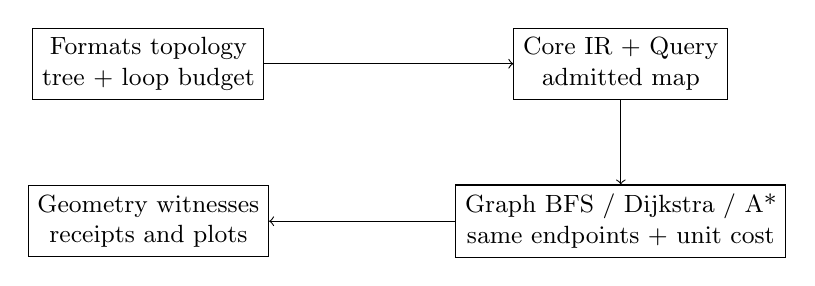
\begin{tikzpicture}[every node/.style={draw,align=center,font=\small}]
\node (g) at (0,0) {Formats topology\\tree + loop budget};
\node (ir) at (6,0) {Core IR + Query\\admitted map};
\node (s) at (6,-2) {Graph BFS / Dijkstra / A*\\same endpoints + unit cost};
\node (r) at (0,-2) {Geometry witnesses\\receipts and plots};
\draw[->] (g)--(ir);\draw[->] (ir)--(s);\draw[->] (s)--(r);
\end{tikzpicture}

\end{document}
